% figure1_propB.tex — Proposal B: labeled-arrow + zoom.
% (a) System overview: workflow lane on top with concrete events, large Active
%     KV cache rectangle in the middle, Host buffer rectangle (dashed orange
%     group) at the bottom. RepairKV is a labeled UP-arrow from Host -> Active.
%     Signal s enters that arrow from above. (No internal modules visible.)
% (b) Expanded view of the RepairKV arrow: Host (left, denser chip grid) ->
%     RepairKV pill (center, single labeled box) -> Active (right, base + 3
%     teal promoted chips appended). Signal s enters pill from above.
%     Ghost outlines in Host show where the K rows came from.
% Shared preamble for standalone Figure 1 variants.
\documentclass[border=8pt,tikz]{standalone}
\usepackage{amsmath}
\usepackage{amssymb}
\usepackage{tikz}
\usetikzlibrary{arrows.meta,positioning,calc,fit,shapes.geometric,backgrounds}
\usepackage{xcolor}
\usepackage[T1]{fontenc}
\usepackage{mathptmx}
\newcommand{\repairkv}{\textsc{RepairKV}}
\newcommand{\bbase}{\ensuremath{B_{\mathrm{base}}}}
\newcommand{\bmatch}{\ensuremath{B_{\mathrm{match}}}}

\begin{document}
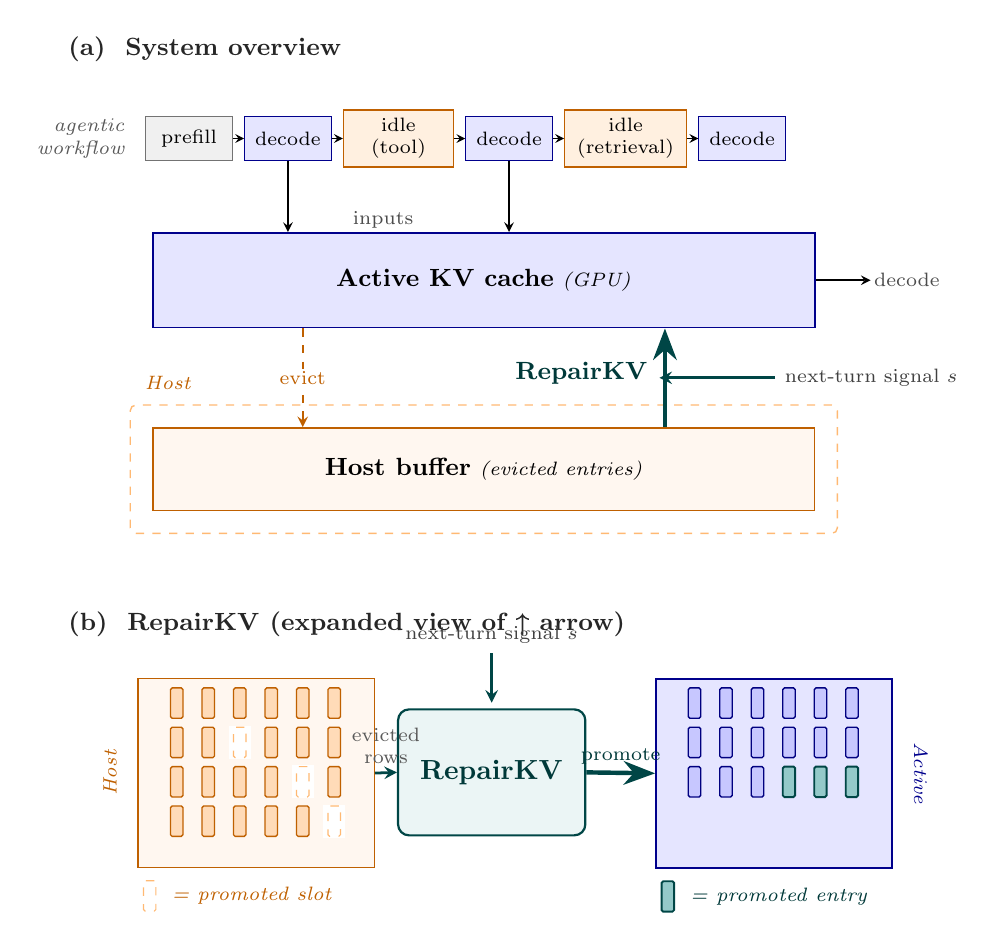
\begin{tikzpicture}[
  >=latex, line width=0.4pt,
  font=\small,
  % --- shared block styles ---
  box/.style={draw=black, fill=white, line width=0.5pt,
              inner sep=5pt, align=center, minimum height=0.85cm},
  active/.style={draw=blue!55!black, fill=blue!10, line width=0.7pt,
                 align=center},
  host/.style={draw=orange!75!black, fill=orange!6, line width=0.5pt,
               align=center},
  % workflow event styles (different colors per event type)
  evprefill/.style={draw=black!55, fill=black!6,  line width=0.4pt,
                    inner sep=3pt, align=center, font=\scriptsize,
                    minimum height=0.55cm},
  evdecode/.style={draw=blue!55!black, fill=blue!10, line width=0.4pt,
                   inner sep=3pt, align=center, font=\scriptsize,
                   minimum height=0.55cm},
  evidle/.style={draw=orange!75!black, fill=orange!12, line width=0.4pt,
                 inner sep=3pt, align=center, font=\scriptsize,
                 minimum height=0.55cm},
  % arrows
  arr/.style={->, line width=0.55pt, draw=black, >=stealth},
  evictarr/.style={->, line width=0.7pt, draw=orange!75!black,
                   dashed, >=stealth},
  rkvarr/.style={-{Stealth[length=4mm,width=3mm]}, line width=1.6pt,
                 draw=teal!55!black},
  thinrkvarr/.style={->, line width=1.0pt, draw=teal!55!black, >=stealth},
  arrlabel/.style={font=\scriptsize, text=black!70, fill=white, inner sep=1pt},
  rkvlabel/.style={font=\bfseries\small, text=teal!45!black,
                   fill=white, inner sep=2pt},
  groupbox/.style={draw=orange!55, dashed, line width=0.5pt,
                   rounded corners=2pt},
  grouplabel/.style={font=\scriptsize\itshape, text=orange!75!black},
  panellabel/.style={font=\bfseries\small, text=black!85},
  paneltitle/.style={font=\scriptsize, text=black!75},
  rowlabel/.style={font=\itshape\scriptsize},
  % chip styles for (b)
  chip/.style={rounded corners=0.6pt, minimum width=4.5pt, minimum height=11pt,
               inner sep=0pt, line width=0.5pt},
  gpuchip/.style={chip, draw=blue!50!black, fill=blue!22},
  hostchip/.style={chip, draw=orange!75!black, fill=orange!28},
  promchip/.style={chip, draw=teal!55!black, fill=teal!42, line width=0.7pt},
  ghostchip/.style={chip, draw=orange!55, fill=white, dashed, line width=0.4pt},
  rkvpill/.style={draw=teal!55!black, fill=teal!8, line width=0.8pt,
                  rounded corners=4pt, inner sep=8pt, align=center,
                  font=\bfseries, text=teal!45!black,
                  minimum width=1.6cm, minimum height=1.6cm},
  signaltxt/.style={font=\scriptsize, text=black!75}
]
  % =================================================================
  % Common horizontal extent: x = 0.4 (left edge of content) to ~10.6
  % =================================================================

  % =================================================================
  % Panel (a) — System overview (high-level block diagram)
  % Layout (from top to bottom):
  %   y =  4.7   panel label "(a)"
  %   y =  3.7   workflow lane with event chips
  %   y =  1.6   Active KV cache (large blue rectangle)
  %   y = -1.0   Host buffer (orange rectangle inside dashed group)
  % Vertical arrows on the LEFT half: workflow -> active (inputs)
  % Vertical arrows on the MIDDLE-RIGHT: active -> host (evict, dashed orange)
  %                                       host -> active (RepairKV, teal bold)
  % Side arrow on the RIGHT: active -> decode out
  % =================================================================
  \node[panellabel, anchor=south west] at (0, 4.7)
       {(a)\,\, System overview};

  % --- Workflow lane (top) ---
  % Six events left-to-right inside a thin enclosing rectangle.
  \node[evprefill, minimum width=1.10cm, anchor=west]
       (e1) at (1.10, 3.85) {prefill};
  \node[evdecode, minimum width=1.10cm, right=4pt of e1] (e2) {decode};
  \node[evidle,   minimum width=1.40cm, right=4pt of e2]
       (e3) {idle\\(tool)};
  \node[evdecode, minimum width=1.10cm, right=4pt of e3] (e4) {decode};
  \node[evidle,   minimum width=1.55cm, right=4pt of e4]
       (e5) {idle\\(retrieval)};
  \node[evdecode, minimum width=1.10cm, right=4pt of e5] (e6) {decode};

  % thin connecting arrows between events
  \foreach \a/\b in {e1/e2, e2/e3, e3/e4, e4/e5, e5/e6}{
    \draw[arr, line width=0.4pt] (\a.east) -- (\b.west);
  }

  % lane label on the left (use align=right to allow the line break)
  \node[font=\scriptsize\itshape, text=black!65, anchor=east, align=right]
       at ([xshift=-4pt]e1.west) {agentic\\workflow};

  % --- Active KV cache (middle) ---
  % Spans almost the full extent so it's clearly the largest rectangle.
  \node[active, minimum width=8.4cm, minimum height=1.20cm,
        anchor=center] (active) at (5.40, 2.05)
       {\textbf{Active KV cache}\,\,\textit{\scriptsize(GPU)}};

  % --- Host buffer (bottom) inside dashed orange group ---
  \node[host, minimum width=8.4cm, minimum height=1.05cm,
        anchor=center] (hostbox) at (5.40, -0.35)
       {\textbf{Host buffer}\,\,\textit{\scriptsize(evicted entries)}};
  \node[groupbox, fit=(hostbox), inner xsep=8pt, inner ysep=8pt]
       (hgroup) {};
  \node[grouplabel, anchor=south west]
       at ([xshift=2pt, yshift=2pt]hgroup.north west) {Host};

  % --- Arrows: workflow -> Active (inputs, on the LEFT side only) ---
  % Drop straight down from the leftmost decode events into the active box.
  \draw[arr] (e2.south) -- (e2.south |- active.north);
  \draw[arr] (e4.south) -- (e4.south |- active.north);
  \node[arrlabel, anchor=south]
       at ([xshift=-1.6cm]e4.south |- active.north) {inputs};

  % --- Active -> Host: evict (dashed orange, on the LEFT side) ---
  \draw[evictarr]
       ([xshift=-2.3cm]active.south) -- ([xshift=-2.3cm]hostbox.north)
       node[arrlabel, text=orange!75!black, pos=0.5] {evict};

  % --- Host -> Active: RepairKV (teal, bold, on the RIGHT side) ---
  % This is the labeled arrow that panel (b) expands.
  \coordinate (rkvStart) at ([xshift=2.3cm]hostbox.north);
  \coordinate (rkvEnd)   at ([xshift=2.3cm]active.south);
  \draw[rkvarr] (rkvStart) -- (rkvEnd);
  \node[rkvlabel, anchor=east]
       at ([xshift=-4pt]$ (rkvStart)!0.55!(rkvEnd) $) {\repairkv{}};

  % --- Signal s entering the RepairKV arrow from the right ---
  % The rkv arrow lives between Host (y~-0.35) and Active (y~1.45).
  % Drop a short arrow from the right side into the midpoint of the rkv arrow
  % so the signal-s label sits clearly outside both the active box and the
  % evict path.
  \coordinate (rkvMid)  at ($ (rkvStart)!0.5!(rkvEnd) $);
  \coordinate (sJoin)   at ([xshift=-2pt]rkvMid);
  \draw[thinrkvarr]
       ([xshift=1.4cm]rkvMid) -- (sJoin);
  \node[signaltxt, anchor=west]
       at ([xshift=1.4cm]rkvMid) {next-turn signal $s$};

  % --- Side arrow: decode exiting Active to the right ---
  \draw[arr] (active.east) -- ++(0.7,0)
       node[arrlabel, anchor=west, fill=none] {decode};

  % =================================================================
  % Panel (b) — Expanded view of the RepairKV arrow
  % Layout: Host (LEFT) -> RepairKV pill (CENTER) -> Active (RIGHT)
  %         Signal s enters pill from above.
  %         Same horizontal extent as (a): x in [0.4, 10.6].
  % =================================================================
  \node[panellabel, anchor=south west] at (0, -2.6)
       {(b)\,\, \repairkv{} (expanded view of \textuparrow\ arrow)};

  % --- Host buffer (LEFT region) with dense chip grid ---
  \node[host, minimum width=3.0cm, minimum height=2.4cm,
        anchor=north west] (hostB) at (1.0, -3.0) {};
  \node[rowlabel, text=orange!75!black, anchor=south, rotate=90]
       at ([xshift=-4pt]hostB.west) {Host};

  % 4 rows x 6 cols = 24 host chips, with 3 ghost-outlined "evicted positions"
  \foreach \i in {1,...,6}{
    \foreach \r in {0,1,2,3}{
      \pgfmathsetmacro{\xh}{0.40*\i + 0.10}
      \pgfmathsetmacro{\yh}{-0.32 - 0.50*\r}
      \node[hostchip] at ([xshift=\xh cm, yshift=\yh cm]hostB.north west) {};
    }
  }
  % overlay 3 ghost chips at chosen positions: (3,1), (5,2), (6,3)
  \pgfmathsetmacro{\xGa}{0.40*3 + 0.10} \pgfmathsetmacro{\yGa}{-0.32 - 0.50*1}
  \pgfmathsetmacro{\xGb}{0.40*5 + 0.10} \pgfmathsetmacro{\yGb}{-0.32 - 0.50*2}
  \pgfmathsetmacro{\xGc}{0.40*6 + 0.10} \pgfmathsetmacro{\yGc}{-0.32 - 0.50*3}
  \fill[white] ([xshift=\xGa cm - 4pt, yshift=\yGa cm - 6pt]hostB.north west)
       rectangle ([xshift=\xGa cm + 4pt, yshift=\yGa cm + 6pt]hostB.north west);
  \fill[white] ([xshift=\xGb cm - 4pt, yshift=\yGb cm - 6pt]hostB.north west)
       rectangle ([xshift=\xGb cm + 4pt, yshift=\yGb cm + 6pt]hostB.north west);
  \fill[white] ([xshift=\xGc cm - 4pt, yshift=\yGc cm - 6pt]hostB.north west)
       rectangle ([xshift=\xGc cm + 4pt, yshift=\yGc cm + 6pt]hostB.north west);
  \node[ghostchip] (gA) at ([xshift=\xGa cm, yshift=\yGa cm]hostB.north west) {};
  \node[ghostchip] (gB) at ([xshift=\xGb cm, yshift=\yGb cm]hostB.north west) {};
  \node[ghostchip] (gC) at ([xshift=\xGc cm, yshift=\yGc cm]hostB.north west) {};

  % Small legend BELOW the host box so the ghost chip + label don't overlap
  % the dense host grid.
  \node[ghostchip, anchor=west] (legendGhost)
       at ([xshift=2pt, yshift=-10pt]hostB.south west) {};
  \node[font=\scriptsize\itshape, text=orange!75!black, anchor=west]
       at ([xshift=2pt]legendGhost.east) {= promoted slot};

  % --- RepairKV pill (CENTER) ---
  \node[rkvpill, anchor=center] (rkv) at (5.5, -4.20)
       {\repairkv};

  % --- Active KV cache (RIGHT region) with chips ---
  \node[active, minimum width=3.0cm, minimum height=2.4cm,
        anchor=north east] (gpuB) at (10.6, -3.0) {};
  % Place the rotated label on the EAST side so it doesn't collide with the
  % incoming promote arrow.
  \node[rowlabel, text=blue!55!black, anchor=south, rotate=-90]
       at ([xshift=4pt]gpuB.east) {Active};

  % Layout chips inside Active:
  %   row 0: 6 base blue chips
  %   row 1: 6 base blue chips
  %   row 2: 6 base blue chips (so 18 base, but we want 5-7 base + 3 teal)
  % Spec said 5-7 base + 3 teal -> render 6 base + 3 teal in a single tidy row,
  % then a few more base above to fill out the rectangle visually.
  % Use 2 rows of 6 base = 12 base + 1 row of 3 teal at the bottom-right.
  \foreach \i in {1,...,6}{
    \foreach \r in {0,1}{
      \pgfmathsetmacro{\xc}{0.40*\i + 0.10}
      \pgfmathsetmacro{\yc}{-0.32 - 0.50*\r}
      \node[gpuchip] at ([xshift=\xc cm, yshift=\yc cm]gpuB.north west) {};
    }
  }
  % 3 base on the bottom-left and 3 teal on the bottom-right (the new ones)
  \foreach \i in {1,2,3}{
    \pgfmathsetmacro{\xc}{0.40*\i + 0.10}
    \pgfmathsetmacro{\yc}{-0.32 - 0.50*2}
    \node[gpuchip] at ([xshift=\xc cm, yshift=\yc cm]gpuB.north west) {};
  }
  \foreach \i in {4,5,6}{
    \pgfmathsetmacro{\xc}{0.40*\i + 0.10}
    \pgfmathsetmacro{\yc}{-0.32 - 0.50*2}
    \node[promchip] (gT\i) at ([xshift=\xc cm, yshift=\yc cm]gpuB.north west) {};
  }

  % Legend BELOW the active box: promoted (teal) chip + label.
  \node[promchip, anchor=west] (legendProm)
       at ([xshift=2pt, yshift=-10pt]gpuB.south west) {};
  \node[font=\scriptsize\itshape, text=teal!45!black, anchor=west]
       at ([xshift=2pt]legendProm.east) {= promoted entry};

  % --- Arrows: Host -> pill (input), pill -> Active (output, teal) ---
  \draw[thinrkvarr]
       (hostB.east) -- (rkv.west);
  \draw[rkvarr]
       (rkv.east) -- (gpuB.west);
  % Labels placed slightly above the arrows (anchor=south, yshift=2pt) and
  % use align=center so the line break renders correctly without collision.
  \node[font=\scriptsize, text=black!65, anchor=south, align=center,
        inner sep=1pt]
       at ([yshift=2pt]$ (hostB.east)!0.5!(rkv.west) $)
       {evicted\\rows};
  \node[font=\scriptsize, text=teal!45!black, anchor=south, inner sep=1pt]
       at ([yshift=2pt]$ (rkv.east)!0.5!(gpuB.west) $) {promote};

  % --- Signal s entering pill from above ---
  \draw[thinrkvarr]
       ([yshift=0.7cm]rkv.north) -- ([yshift=2pt]rkv.north);
  \node[signaltxt, anchor=south]
       at ([yshift=0.7cm]rkv.north) {next-turn signal $s$};

\end{tikzpicture}
\end{document}
